\documentclass[12pt ,a4paper ]{article}

\usepackage[utf8]{inputenc}
\usepackage[T1]{fontenc}      % caractères français
\usepackage[francais]{babel}  %langue
\usepackage[left=2.3cm,right=2.5cm,bottom=2.5cm,top=2.3cm]{geometry}   % marges
\usepackage{verbatim}
\usepackage{float}
\usepackage{graphicx}         % images
\usepackage{verbatim}
\usepackage{multicol}
\usepackage{titlesec}


                           
\begin{document}
	\begin{titlepage}
		
		\vspace{0.5cm}
		\begin{center}		
			{\Large  Master 1 Informatique}
		\end{center}
		\vspace{1cm}
		
		\rule{1\linewidth}{1.1pt}\newline   %regle
		\begin{center}
			 {\Huge \textbf{Rapport de Projet : Traitement Automatique du Texte en IA}}
		\end{center}
		\rule{1\linewidth}{1.1pt} \\
		
		\begin{center}
		\begin{LARGE}
		\textbf{Sujet :} \\\vspace{0.6cm} Identification des opinions exprimées dans les avis et commentaires d’un ordinateur.
		\end{LARGE}
		\end{center}
		
		\vspace{0.5cm}
		\begin{center}	
				\begin{Large}
				Yann MARTIN D'ESCRIENNE \\ 
				Yohann TOGNETTI \\ 
				\end{Large}
		\end{center}
		\vspace{6cm}
		
		\begin{center}
			{\large « Année universitaire 2020 - 2021 »}
		\end{center}
		

\end{titlepage}

\newpage
\tableofcontents 
				
\newpage


\begin{multicols}{2} 
\section{Introduction}

	\subsection{Présentation générale du projet}
		Dans le cadre de notre cours de Traitement automatique du texte en IA, il nous a été demandé d'effectuer un projet de notre choix impliquant une intelligence artificielle travaillant sur des données textuelles. La restriction sur le sujet se limitant à l'existence d'un jeu de données conséquent.
	
	\subsection{Choix du sujet}
		Notre choix de sujet fut \textbf{l'identification des opinions exprimées dans les avis et commentaires d’un ordinateur.} Plus précisément, comment retrouver parmi un ensemble de commentaires les parties de l'ordinateur visées,  sur quels aspects et quel en est l'avis général qui en ressort. 
		
\section{Description des tâches}
Ce sujet est fortement inspiré du « SemEval-2015 Task 12 » sur la partie « Aspect Based Sentiment Analysis (ABSA): Laptop Reviews » et partage donc le même objectifs avec des simplifications. Les différentes entités et catégories qui vont suivre provienne également des annotations du sujet de SemEval. Chacun des commentaires est fragmentés phrase par phrase afin de faciliter le travail de l'IA. 
		
\subsection{Entités}
\noindent Tout d'abord il s'agit de retrouver dans la phrase le(s) entité(s) ciblée. Elles peuvent être l'ordinateur comme un tout, ses parties physique (clavier, écran..) , des logiciels ou OS (Windows, navigateur, jeux...) ou bien même une compagnie et ses services. (DELL, Apple, le support technique, la livraison..).\\

\noindent\textit{Remarque : } Rien n'interdit d'avoir plusieurs entités dans la même phrase.\\
		
\noindent Voici la liste des entités possible : 
\begin{itemize}
\item DISPLAY (=moniteur, écran), 
\item CPU (=processeur), 
\item MOTHERBOARD (=carte mère),
\item HARDDISC (=disque dur), 
\item MEMORY (=mémoire, RAM), 
\item BATTERY (=batterie), 
\item POWER\_SUPPLY (=chargeur, unité de chargement, cordon d'alimentation, (power) adapteur),
\item KEYBOARD (=touche, clavier, pavé numérique), 
\item MOUSE (=sourie, pavé tactile)
\item FANS\_COOLING (=ventilateur, système de refroidissement), 
\item OPTICAL\_DRIVES (=lecteur CD, DVD ou Blue-ray),
\item PORTS (=USB, HDMI, VGA, lecteur de carte),
\item GRAPHICS (=carte graphique, carte video),
\item MULTIMEDIA\_DEVICES (=son, audio, microphone, webcam, haut-parleur, casque, écouteurs).
\end{itemize}				

\subsection{Catégories}
\noindent Une fois obtenue il faut également trouver sur quelle(s) catégorie(s) de l'entité le commentaire porte. Cela peut être un aspect général , sa prise en main, ses performances, son design et ses fonctionnalités, etc... \\

\noindent\textit{Remarque : }Là encore, rien n'interdit d'aborder plusieurs catégorie pour la même entité au sein d'une même phrase.\\

\noindent Voici la liste des catégories possible : 
\begin{itemize}
\item GENERAL, 
\item PRICE (=prix), 
\item QUALITY (=qualité), 
\item DESIGN\_FEATURES (=design et fonctionnalités),
\item OPERATION\_PERFORMANCE, 
\item USABILITY (=ergonomie, prise en main), 
\item PORTABILITY (=portabilité),
\item CONNECTIVITY (=connectivité), 
\item MISCELLANEOUS (=divers).
\end{itemize}	

\paragraph{} 
\noindent L'entité E et la catégorie C qui s'y rapporte forme ainsi un couple E\#C. \\

\noindent\textit{Remarque : }Il est à noter la possibilité qu'aucun couple E\#C ne se rapporte à une phrase d'un commentaire.

\subsection{Polarité}
Enfin, chaque phrase (et non chaque couple E\#C comme dans le sujet de SemEval) se verra attribuer une polarité. Les valeurs de cette polarité sont : \textbf{negative} pour les phrases soulignant des défauts ou de mauvais avis, \textbf{positive} pour celles qui au contraire mettent en valeur des points ou des avis positif, \textbf{neutral} lorsque la phrase ne met pas d'opinion en avant et donne par exemple un conseil et finalement \textbf{mixed} pour les textes critiquant un aspect de l'ordinateur mais appréciant un autre. 

\section{Jeux de données}
Les jeux de données se divisent en deux groupes : le jeu de données d'entrée correspondant à ce que l'IA va utiliser pour s'entrainer et celui de test sur lequel les mesures seront effectuées. Tout deux proviennent du site du SemEval. 

\subsection{Structure des jeux de données}
\noindent Ce sont tout deux des documents XML possédant la structure suivante (simplifiée) :  

\begin{figure}[H]
\begin{center}
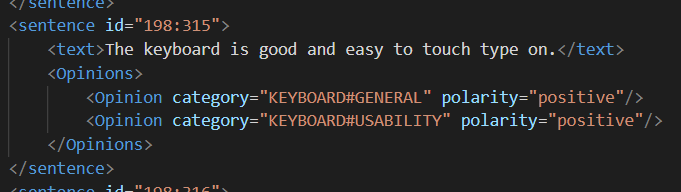
\includegraphics[scale=0.55]{xml_struct.png}
\caption{\small{structure du fichier XML}}
\end{center}
\end{figure}

\subsection{Modification des jeux de données}
Suite à notre implémentation de notre IA qui sera décrite dans le chapitre suivant, de nombreux problèmes nous ont forcés à ajouter nous même des phrases dans le jeu de données d'entrainement.\\

En effet notre IA répond de la présence ou non de chaque couple E\#C dans la phrase actuelle pour chaque combinaison d'entité E et catégorie C. Cela se traduit par une nécessité de nombreuses données appartenant à chacun des couples pouvant apparaitre afin d'obtenir une fonction d'évaluation optimale. 

\paragraph{}
\noindent Environ 350 phrases ont été ajoutées, toutes sont la section 'sentences' d'\textbf{ID 198}. Certaines proviennent d'avis de consommateur sur les ordinateur portables les plus commentés sur Amazon (en anglais), notamment pour les phrases portant sur les clavier, écran, pavé tactile et batterie. Nous avons rédigés le reste pour les catégories plus complexe et moins abordées en générale. Par exemple la qualité des lecteurs DVD ou bien l'ergonomie des OS. \\ 

\noindent \textit{Remarque : } Il est à noté que certain couple n'apparaissent ni dans les données d'entrainement, ni dans les données de test. Par simplification, ces couples ont été ignorés et aucunes phrases n'est étiquetées avec.

\begin{figure*}[ht]
    \begin{center}
        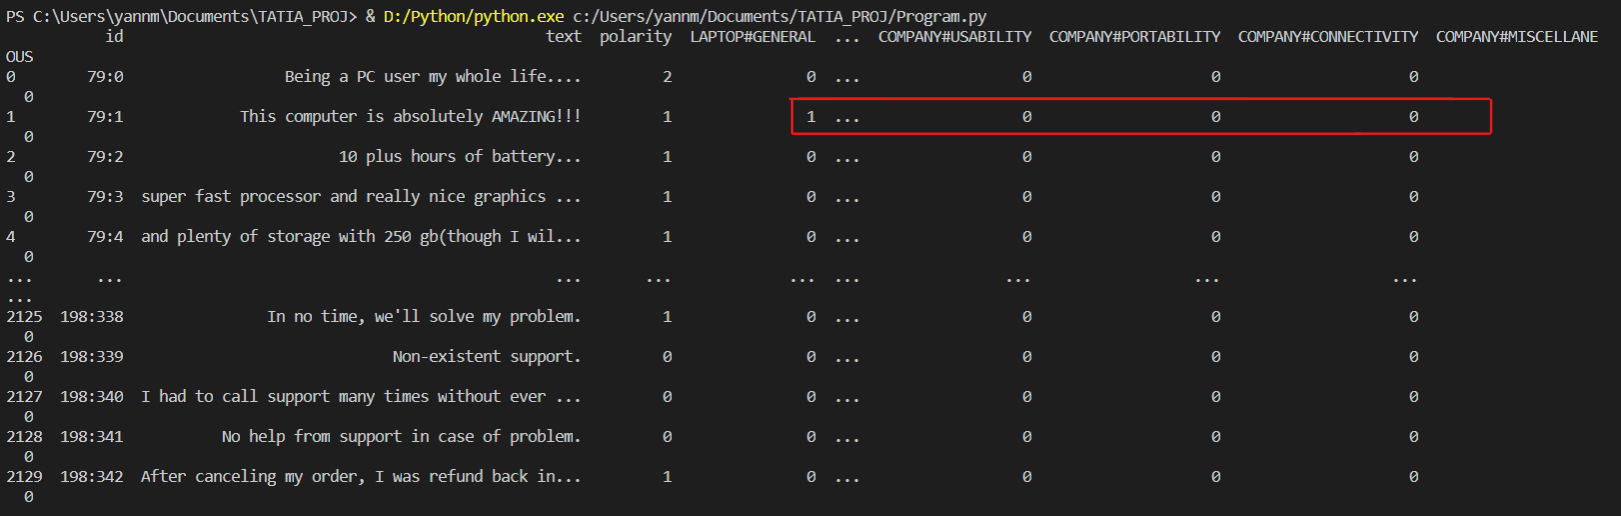
\includegraphics[width=1\textwidth]{first_dataf.png}
    \end{center}
\caption{\small{dataframe du fichier XML}}
\end{figure*}

\newpage
\section{Implémentation de l'algorithme}
Notre algorithme est développé en python. Il se divise en 4 fichiers de code ayant chacun un rôle précis dans l'implémentation de l'algorithme d'apprentissage. 

\subsection{DataInitializer.py}
Ce fichier permet de lire un documents XML du jeu de données et regroupe les informations essentielles dans un dataframe de la librairie \textit{panda}. Chacune des phrases correspondent à une ligne dans le dataframe. \\

\noindent Il vient tout d'abord récupérer l'ID et le texte de chaque phrase. \\

\noindent Ensuite il récupère chaque couple E\#C et transforme le tout en un vecteur binaire ayant des 1 uniquement aux colonnes correspondant au couple comme sur l'image ci-dessus. Étant donné le nombre de couples possible, il s'agit d'une vecteur à 197 dimensions comportant majoritairement des 0.\\

\noindent Finalement, le programme récupérera la polarité de chaque couple E\#C et en conclue une polarité générale de la phrase selon les règles suivantes :
\begin{enumerate}
\item \textbf{\small{neutral + X = X, X une polarité. }}
\item \textbf{\small{positive + negative = mixed.}}
\item \textbf{\small{mixed + X = mixed, X une polarité.}}
\end{enumerate}

\noindent Cette polarité général est ensuite convertie en entier:

\noindent \textbf{0=negative, 1=positive, 2=neutral, 3=mixed.}

\subsection{PreProcessing.py}
Ce fichier permet d'effectuer un pré traitement sur les textes du premier data frame afin de facilité le travail d'apprentissage de l'IA.\\

\noindent Tout d'abord le texte va être mit en minuscule afin de ne pas différencier des mots n'ayant pas la même casse. Ensuite chacun de ses mots (y compris la ponctuation) va être transformé en \textbf{« token »}. De ces tokens sera retiré la ponctuation ainsi que ce que l'on appelle les \textbf{STOPWORDS}. Ce sont les mots n'ayant pas de grande valeurs syntaxique comme les déterminants, adjectifs possessifs, conjonctions de coordination, verbes communs (être, avoir)...\\

\noindent L'étape suivante consiste à effectuer une \textbf{lemmatisation} sur chacun des tokens. La lemmatisation est un traitement lexical qui consiste à appliquer aux verbes, substantifs, adjectifs... un codage renvoyant à leur entrée lexicale commune, leur « forme canonique ».\\\\

\noindent \textit{Exemple :}\\
Les / la\\
étoiles /étoile\\
claires / clair\\
luisent / luire\\
noire / noir\\

\noindent Voici une image des phrases du dataframe précédent où celles-ci ont été pré-traitées : 
\begin{figure}[H]
    \begin{center}
        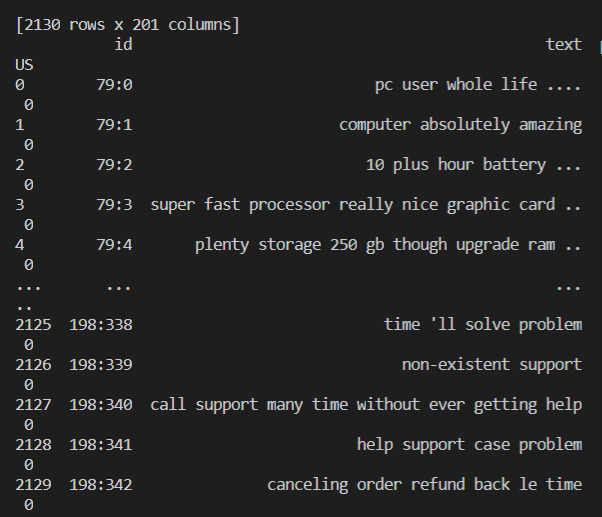
\includegraphics[scale=0.62]{pretrait_dataf.png}
    \end{center}
\caption{\small{Phrases pré-traitées}}
\end{figure}

\subsection{Classify.py}
Ce fichier a pour fonction de créer un classificateur pour chaque classe qui a des donnée pour s'entrainer. L'intégralité de ce fichier utilise principalement la librairie sklearn qui est une librairie complète pour l'apprentissage d'une ia.\\

\noindent La première opération a faire pour pouvoir créer un classificateur, c'est de transformer en vecteur les phrase. Pour cela, nous avons utiliser TfidfVectorizer de la librairie sklearn. Au niveau des paramètre, nous avons décidé d'utiliser la norme "l2" et d'utiliser des ngram entre 1 et 8. Une fois crée nous avons entrainer ce vectoriseur avec les commentaire de notre jeu de d'entrainement.\\

Ensuite, nous pouvont commencer la classification. Pour celle-ci nous avons décidé d'utiliser la méthode one-versus-rest (« une contre le reste »). Cette méthode consiste a  traiter chaque classe indépendamment des autre. Du coup notre première étape pour chaque catégorie est d'équilibre le nombre de données entre les élément qui appartiennent a notre classe et eu qui ne le sont pas. Pour cela nous avons utiliser ADASYN qui nous permet de rajouter des vecteur entre les divers point.\\

Après avoir fait cela, il nous reste plus qua entrainer un classificateur. Nous avons utiliser le classificateur OneVsRestClassifier avec comme solver "sag", le pois de chaque classe en équilibré avec un nombre d'itération max de 1000. Avec ce classificateur, nous avons plus qu'a l'entrainer et le stocker dans un dictionnaire.\\

La dernière fonction de cette classe est la prédiction un dataframe test. Pour ce faire, a l'aide du vectorisateur et des classificateur, il nous suffit de vectoriser chaque phrase et d'appeler pour chacune l'intégralité de classificateur stocker dans le dictionnaire pour savoir a quel classe appartient chaque commentaire.

\subsection{PlotResult.py}
Cette classe utilise la libraire matplotlib de python pour pouvoir voir les résultat sous forme de graphe, ce qui permet d'avoir une vision d'ensemble de la classification effectué. Grâce a cela nous pouvons voir instantanément la precision de notre classification pour chaque classe.
Nos graphe sont orienté sur les moyenne non pondéré car comme il y a peut de phrase dans le jeu de test, il nous suffirait de répondre que chaque phrase n'appartiens a aucune classe pour avoir un score de 99\%, ce qui n'a aucun intérêt pour notre projet.

\end{multicols}
\end{document}